\def\documentauthor{Carlos Salinas}
\def\documenttitle{MA571 Homework \hwnum}
\def\hwnum{13}
\def\shorttitle{MA571 HW \hwnum}
\def\coursename{MA571}
\def\documentsubject{point-set topology}
\def\authoremail{salinac@purdue.edu}

\documentclass[article,oneside,10pt]{memoir}
\usepackage{geometry}
\usepackage[dvipsnames]{xcolor}
\usepackage[
    breaklinks,
    bookmarks=true,
    colorlinks=true,
    pageanchor=false,
    linkcolor=black,
    anchorcolor=black,
    citecolor=black,
    filecolor=black,
    menucolor=black,
    runcolor=black,
    urlcolor=black,
    hyperindex=false,
    hyperfootnotes=true,
    pdftitle={\shorttitle},
    pdfauthor={\documentauthor},
    pdfkeywords={\documentsubject},
    pdfsubject={\coursename}
    ]{hyperref}

% Use symbols instead of numbers
\renewcommand*{\thefootnote}{\fnsymbol{footnote}}

%% Math
\usepackage{amsthm}
\usepackage{amssymb}
\usepackage{mathtools}
% \usepackage{unicode-math}

%% PDFTeX specific
\usepackage[mathcal]{euscript}
\usepackage{mathrsfs}

\usepackage[LAE,LFE,T2A,T1]{fontenc}
\usepackage[utf8]{inputenc}
\usepackage[farsi,french,german,spanish,dutch,russian,swedish,english]{babel}
\babeltags{pa=farsi,
           fr=french,
           de=german,
           es=spanish,
           nl=dutch,
           ru=russian,
           sv=swedish,
           en=english}
\def\spanishoptions{mexico}

\selectlanguage{english}

\newcommand{\textfa}[1]{\beginR\textpa{#1}\endR}

\usepackage{cmap}
\usepackage{CJKutf8}
\newcommand{\textha}[1]{\begin{CJK}{UTF8}{mj}#1\end{CJK}}
\newcommand{\textni}[1]{\begin{CJK}{UTF8}{min}#1\end{CJK}}
\newcommand{\textzh}[1]{\begin{CJK}{UTF8}{bsmi}#1\end{CJK}}

\usepackage{graphicx}
\graphicspath{{figures/}}

% Misc
\usepackage{microtype}
\usepackage{multicol}
\usepackage[inline]{enumitem}
\usepackage{listings}
\usepackage{mleftright}
\mleftright

%% Theorems and definitions
%% remove parentheses
\makeatletter
\def\thmhead@plain#1#2#3{%
  \thmname{#1}\thmnumber{\@ifnotempty{#1}{ }\@upn{#2}}%
  \thmnote{ {\the\thm@notefont\textbf{#3}}}}
\let\thmhead\thmhead@plain
\makeatother

\theoremstyle{plain}
\newtheorem{theorem}{Theorem}
\newtheorem{proposition}[theorem]{Proposition}
\newtheorem{corollary}[theorem]{Corollary}
\newtheorem{claim}[theorem]{Claim}
\newtheorem{lemma}[theorem]{Lemma}
\newtheorem{axiom}[theorem]{Axiom}

\newtheorem*{corollary*}{Corollary}
\newtheorem*{claim*}{Claim}
\newtheorem*{lemma*}{Lemma}
\newtheorem*{proposition*}{Proposition}
\newtheorem*{theorem*}{Theorem}

\theoremstyle{definition}
\newtheorem{definition}{Definition}
\newtheorem{example}{Examples}
\newtheorem{examples}[example]{Examples}
% \newtheorem{exercise}{Exercise}[section]
% \newtheorem{problem}[exercise]{Problem}

\newcounter{problem}
\newenvironment{problem}[1][]% environment name
{% begin code
  \stepcounter{problem}
  \par\vspace{\baselineskip}\noindent
  \ifx &#1&%
  {\normalfont\Large\bfseries\scshape Problem~\hwnum.\theproblem}
  \global\def\exercisename{Problem~\hwnum.\theproblem}%
  \else
  {\normalfont\Large\bfseries\scshape Problem~\hwnum.\theproblem~(#1)}
  \global\def\exercisename{Problem~\hwnum.\theproblem(#1)}
  \fi
  \par\vspace{\baselineskip}%
  \noindent\ignorespaces
}%
{% end code
  \par\vspace{\baselineskip}%
  \noindent\ignorespacesafterend
}

\newtheorem*{definition*}{Definition}
\newtheorem*{example*}{Examples}
\newtheorem*{examples*}{Examples}
\newtheorem*{exercise*}{Exercise}
\newtheorem*{problem*}{Problem}

\theoremstyle{remark}
\newtheorem{remark}{Remark}
\newtheorem{remarks}[remark]{Remarks}
\newtheorem{observation}[remark]{Observation}
\newtheorem{observations}[remark]{Observations}

\newtheorem*{remark*}{**Remark**}
\newtheorem*{remarks*}{**Remarks**}
\newtheorem*{observation*}{**Observation**}
\newtheorem*{observations*}{**Observations**}

%% Redefinitions & commands
% \newcommand\restr[2]{{% we make the whole thing an ordinary symbol
%   \left.\kern-\nulldelimiterspace % automatically resize the bar with \right
%   {#1} % the function
%   % \vphantom{\big|} % pretend it's a little taller at normal size
%   \right|{#2} % this is the delimiter
%   }}

\newcommand\minus{\smallsetminus}
\newcommand{\nsubset}{\ensuremath{\not\subset}}
\newcommand{\nsupset}{\ensuremath{\not\supset}}

\renewcommand\qedsymbol{\ensuremath{\null\hfill\blacksquare}}

%% Commands and operators
\DeclareMathOperator{\diam}{diam}
\DeclareMathOperator{\id}{id}
\DeclareMathOperator{\im}{im}
\DeclareMathOperator{\Int}{int}
\DeclareMathOperator{\Cl}{cl}

\newcommand{\CC}{\mathbb{C}}
\newcommand{\NN}{\mathbb{N}}
\newcommand{\QQ}{\mathbb{Q}}
\newcommand{\RR}{\mathbb{R}}
\newcommand{\ZZ}{\mathbb{Z}}

% Renewcommands
% \renewcommand\setminus{\smallsetminus}
% \renewcommand\phi{\varphi}
% \renewcommand\epsilon{\varepsilon}

\begin{document}
\frontmatter
\aliaspagestyle{title}{empty}
\pagestyle{title}
\author{\href{mailto:\authoremail}{\documentauthor}}
\title{\documenttitle}
\date{\today}
\maketitle
\cleartooddpage

\makeoddhead{headings}
        {\small{\MakeUppercase{\itshape\documentauthor}}}
        {}
        {\small{\MakeUppercase{\itshape\exercisename}}}
\makeoddfoot{headings}{{\itshape\documenttitle}}
                      {}
                      {\thepage}
\makeevenhead{headings}
        {\small{\MakeUppercase{\itshape\documentauthor}}}
        {}
        {\small{\MakeUppercase{\itshape\exercisename}}}
\makeevenfoot{headings}{{\itshape\documenttitle}}
                      {}
                      {\thepage}
\makeheadrule{headings}{\textwidth}{.25pt}
% \makerunningwidth{headings}{1.15\textwidth}
\pagestyle{headings}

\mainmatter
% \setcounter{theorem}{16}
\begin{problem}[Munkres \S68, Ex.\,1]
Check the details of Example 1.
\end{problem}
\begin{proof}
The following is the statement of Example 1 as found in the book:
\begin{example*}[1]
Consider the group $P$ of bijections of the set $\{0,1,2\}$ with
itself. For $i=1,2$, define an element $\pi_1$ of $P$ by setting
$\pi_i(i)=i-1$ and $\pi_i(i-1)=i$ and $\pi_i(j)=j$ otherwise. Then $\pi_i$
generates a subgroup $G_i$ of $P$ of order $2$. The group $G_1$ and $G_2$
generate $P$, as you can check. But $P$ is not their free product. The
reduced words $(\pi_1,\pi_2,\pi_1)$ and $(\pi_2,\pi_1,\pi_2)$, for
instance, represent the same element of $P$.
\end{example*}
We need to check two claims (i) that $G_1$ and $G_2$, as defined above,
generate $P$ and (ii) that $P\neq G_1*G_2$, i.e., show that
$(\pi_1,\pi_2,\pi_1)=(\pi_2,\pi_1,\pi_2)$. Let us deal with (i) first. We
show that $\langle G_1,G_2 \rangle=P$. Our strategy is the following, by
the pigeon-hole principle, it suffices to show that $\langle  G_1,G_2
\rangle\subset P$ and that $|\langle G_1,G_2\rangle|=|P|$. Since
$G_1,G_2<P$, i.e., $G_1$ and $G_2$ are subgroups of $P$, the group
generated by $G_1$ and $G_2$ will be a subgroup of $P$ hence, $\langle
G_1,G_2 \rangle\subset P$. The group $P$ is a well-known group, namely (up
to group isomorphism) $S_3$, and we shall not waste time any time showing
that $|P|=|\{0,1,2\}|=3!=6$, but instead we proceed to showing that
$|\langle G_1,G_2 \rangle|=6$. From the definitions of $G_1$ and $G_2$, we
have at least $3$ in $\langle  G_1,G_2 \rangle$, these are the elements
$1$, $\pi_1$ and $\pi_2$ (the latter two have order $2$, e.g.,
\[
\pi_i^2(j)=
\pi_i\left(
\begin{cases}
i-1&\text{if $j=i$}\\
i&\text{if $j=i-1$}\\
j&\text{otherwise}
\end{cases}\right)
=
\begin{cases}
i&\text{if $j=i$}\\
i-1&\text{if $j=i-1$}\\
j&\text{otherwise}
\end{cases}
\]
which is the identity on $\{0,1,2\}$.) So the elements
$1,\pi_1,\pi_2,\pi_1\pi_2,\pi_2\pi_1,\pi_1\pi_2\pi_1\in\langle
G_1,G_2\rangle$ and all finite strings $\pi_1\pi_2\cdots\pi_i$,
$\pi_2\pi_1\cdots\pi_i$ for that matter. But as a consequence of Lagrange's
theorem, the size of $\langle G_1,G_2\rangle$ must not exceed the size of
$P$ so that we are done when we show that the elements $\pi_1\pi_2$,
$\pi_2\pi_1$ and $\pi_1\pi_2\pi_1$ are distinct elements. First, observe that
\begin{align*}
\pi_2\pi_1(j)&=
\pi_2\left(
\begin{cases}
1&\text{if $j=0$}\\
0&\text{if $j=1$}\\
2&\text{if $j=2$}
\end{cases}
\right)
&
\pi_1\pi_2(j)&=
\pi_1\left(
\begin{cases}
0&\text{if $j=0$}\\
2&\text{if $j=1$}\\
1&\text{if $j=2$}
\end{cases}
\right)
\\
&=
\begin{cases}
2&\text{if $j=0$}\\
0&\text{if $j=1$}\\
1&\text{if $j=2$}
\end{cases}
&&=
\begin{cases}
1&\text{if $j=0$}\\
2&\text{if $j=1$}\\
0&\text{if $j=2$}
\end{cases}
\end{align*}
and, using the computations above,
\[
\pi_1\pi_2\pi_1(j)=
\pi_1\left(
\begin{cases}
2&\text{if $j=0$}\\
0&\text{if $j=1$}\\
1&\text{if $j=2$}
\end{cases}
\right)\\
=
\begin{cases}
2&\text{if $j=0$}\\
1&\text{if $j=1$}\\
0&\text{if $j=2$}
\end{cases}.
\]
Note that none of these elements are equivalent to any of $1$, $\pi_1$ or
$\pi_2$ and are certainly not equal to each other. Moreover, there are six
of these elements and there are no more elements in $P$ since
$|P|=6$. Thus, $\langle G_1,G_2 \rangle=P$.

Lastly, we show that $P\neq G_1*G_2$ since
\[
(\pi_1,\pi_2,\pi_1)=
\pi_1\pi_2\pi_1(j)=
\begin{cases}
2&\text{if $j=0$}\\
1&\text{if $j=1$}\\
0&\text{if $j=2$}
\end{cases}
\]
and
\[
(\pi_2,\pi_1,\pi_2)=
\pi_2\pi_1\pi_2(j)=
\pi_1\left(
\begin{cases}
1&\text{if $j=0$}\\
2&\text{if $j=1$}\\
0&\text{if $j=2$}
\end{cases}
\right)
=
\begin{cases}
2&\text{if $j=0$}\\
1&\text{if $j=1$}\\
0&\text{if $j=2$}
\end{cases}
\]
would imply that $(\pi_1,\pi_2,\pi_1)=(\pi_2,\pi_1,\pi_2)$ in the free
product $G_1*G_2$, but $\pi_1\neq\pi_2$.
\end{proof}
\newpage
\begin{problem}[Munkres \S68, Ex.\,2(a,b,c)]
Let $G=G_1*G_2$, where $G_1$ and $G_2$ are nontrivial groups.
\begin{enumerate}[label=(\alph*)]
\item Show $G$ is not Abelian.
\item If $x\in G$, define the \emph{length} of $x$ to be the length of the
  unique reduced word in the elements of $G_1$ and $G_2$ that represents
  $x$. Show that if $x$ has even length (at least $2$), then $x$ does not
  have finite order. Show that if $x$ has odd length (at least $3$), then
  $x$ is conjugate to an element of shorter length.
\item Show that the only elements of $G$ that have finite order are the
  elements of $G_1$ and $G_2$ that have finite order, and their
  conjugates.
\end{enumerate}
\end{problem}
\begin{proof}
(i) Suppose $G$ is Abelian. Take an element $x\in G_1$ and $y\in G_2$. Then
$(x,y)=(y,x)$. By the definition of a free product (Munkres \S68,
pp.\,413-414) this implies that the word $(x^{-1},y^{-1},x,y)=1$ which
implies that $y^{-1}x=1$, but $y^{-1}\notin G_1$.
\\\\
(ii) Let $x\in G$ be a word of even length. Then $x=(y_1,y_2,...,y_{2k})$
for $k\in\NN$ where the right hand-side is irreducible, i.e., either
$y_i\in G_1$ if $2\mid i$ and $y_j\in G_2$ if $2\nmid j$ or vice-versa
since two consecutive ``letters'' in a word must be from distinct groups or
else we can reduce the word further. Then
$x^2=(y_1,y_2,...,y_{2k},y_1,y_2,...,y_{2k})$ is again irreducible since
$y_{2k}\in G_1$ and $y_1\in G_2$ or vice-versa. It follows by induction
that $x^n\neq 1$ for any finite positive integer $n$.

Now, suppose that $x\in G$ has odd length. Then $x=(y_1,y_2,...,y_{2k+1})$
for $k\in\NN$ where the right hand-side is irreducible. Without loss of
generality, we may assume that $y_1,y_{2k+1}\in G_1$. Then, setting
$y_{2k+1}'\coloneqq y_{2k+1}y_1$, we have
\[
y_1^{-1}xy_1=y_1^{-1}(y_1,y_2,...,y_{2k+1})y_1=(y_2,y_3,...,y_{2k+1}y_1)=(y_2,y_3,...,y_{2k+1}')
\]
which has length $2k$. Thus, $x$ is conjugate to a word of shorter
length.
\\\\
(iii) Suppose that $x\in G$ has finite order. By part (i) the length of $x$
cannot be even. Moreover, if $x$ is of finite order, i.e., if $x^n=1$ for
some positive integer $n$, and $y$ is conjugate to $x$, i.e., there exist
$g\in G$ such that $y=g^{-1}xg$, then
\[
y^n=(g^{-1}xg)^n=(g^{-1}xg)(g^{-1}xg)\cdots(g^{-1}xg)=g^{-1}x^ng=1
\]
so $y$ is of finite order. It remains to show that if $x$ has finite order
then $x$ is a conjugate of an element $y$ of $G_i$, where $i=1,2$. Let
$2k+1$ be the length of $x$. By part (ii), $x$ is conjugate to an element
$y'$ of shorter length. Since $x$ has finite order $y$ has finite order so
by part (i) $y'$ must be of odd length. If $y'$ is of length $1$ we are
done. If not, then $y'$ is conjugate to a word $y''$ of shorter
length with finite order. Since the length of $x$ is finite, this process
must terminate at a word $y$ of length $1$ with finite order.
\end{proof}
\newpage
\begin{problem}[Munkres \S68, Ex.\,3]
Let $G=G_1*G_2$. Given $c\in G$, let $cG_1c^{-1}$ denote the set of all
elements of the form $cxc^{-1}$, for $x\in G_1$. It is a subgroup of $G$;
show that the intersection with $G_2$ is the identity alone.
\end{problem}
\begin{proof}
Suppose $y\in cG_1c^{-1}\cap G_2$. Then $y=cxc^{-1}$ for some $x\in
G_1$ and we have, $c=ycx^{-1}$. Let us deal with the trivial case first. If
$c=1$ then, since $G$ is the free group of $G_1$ and $G_2$, we have $1\cdot
G_1\cdot 1^{-1}=G_1$ so $(1\cdot G_1\cdot 1^{-1})\cap G_2=G_1\cap G_2=1$ by
definition of the free product. Now, suppose $c\neq 1$, say that $c$ is
represented by the unique reduced word $(y_1,...,y_k)$, $k\in\NN$. We show
that for the following cases (i) $y_1,y_k\in G_i$, (ii) $y_1\in G_1$ and
$y_k\in G_2$, or $y_1\in G_2$ and $y_k\in G_1$, $y=1$, i.e., the
intersection $cG_1c^{-1}\cap G_2=1$.

The above three cases can trivially be adapted to just the case where
$y_1,y_k\in G_1$ or $y_1,y_k\in G_2$, so we shall prove the
aforementioned. Assuming $y_1,y_k\in G_1$, $c$ is represented by
$(y_1,...,y_k)$ and $(y,y_1,...,y_k,x^{-1})$ where the latter reduces to
the word $(y,y_1,...,y_kx^{-1})$. Now, by the uniqueness of representation
by reduced word, $(y_1,...,y_k)=(y,y_1,...,y_kx^{-1})$, but the right-hand
side has length $k+1$ and cannot be reduced further unless
$y_kx^{-1}=1$. Suppose that $y_kx^{-1}$ then we have,
$y_1=y,y_2=y_1,...,y_k=y_{k-1}$ which can only happen if $y=1$ and $y_i=1$
for all $i$. But this contradicts the assumption that $c\neq 1$. Thus,
$y=1$ to begin with.

Now, suppose $y_1,y_k\in G_2$, then $c$ is represented by $(y_1,...,y_k)$
and $(y,y_1,...,y_k,x^{-1})$ where the latter reduces to  the word
$(yy_1,...,y_k,x^{-1})$. Now, by the uniqueness of representation by
reduced word, $(y_1,...,y_k)=(yy_1,...,y_k,x^{-1})$, but the right-hand
side has length $k+1$ and cannot be reduced further unless the product
$yy_1=1$. Suppose that $yy_1=1$. Then we have,
$y_2=y_1,,...,y_{k-1}=y_k,y_k=x$. This implies that, since $y_i\notin
G_{\alpha_{i+1}}$, $x=1$ and $y_i=1$ for all $i$. But this contradicts the
assumption that $c\neq 1$. Thus, $y$ must have been $1$ to begin with.
\end{proof}
\newpage
\begin{problem}[A]
\begin{enumerate}[label=(\roman*)]
\item Do the case of p.\,367 \# 9(e) where $h$ and $k$ take $b_0$ to
  $b_0$. (The proof is similar to the proof of Lemma 55.3, (3) $\implies$
  (1), that I gave in class).
\item Let $G$ be a path-connected topological group and let $a\in G$. Prove
  that the map $\varphi\colon G\to G$ defined by $\varphi(g)\coloneqq ag$
  is homotopic to the identity map.
\item Use part (ii) to complete the proof of p.\,367 \# 9(e).
\end{enumerate}
\end{problem}
\begin{proof}
(i) Set $d\coloneqq\deg h$. Suppose that $h(b_0)=k(b_0)=b_0$ and that $\deg
h=\deg k$. Consider the path $f(s)\coloneqq(\cos(2\pi s),\sin(2\pi s))$
from the handout on ``The fundamental group of $S^1$.'' This path is a loop
at $b_0$ ($f(0)=(\cos(2\pi\cdot 0),\sin(2\pi\cdot
0))=(1,0)=(\cos(2\pi),\sin(2\pi))f(1)$) of index $1$ (i.e., the winding
number of $f$ is $1$), hence is a generator for $\pi_1(S^1,b_0)$. Thus, we
have
\[
h_*([f])=d\cdot[f]=k_*([f])
\]
so $h\circ f\simeq_p k\circ f$. Let $H\colon I\times I\to S^1$ denote the
homotopy from $h\circ f$ to $k\circ f$, i.e., the continuous map such that
$H(s,0)=h\circ f(s)$ and $H(s,1)=k\circ f(s)$. Next, by the Problem 9.2
(Munkres \S46, Ex.\,9), we see that the map $(f,\id_I)\colon I\times I\to
S^1\times I$ is a quotient map so that the following diagram commutes
\begin{center}
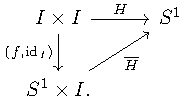
\includegraphics{figures/hw-13-degree-diagram}
\end{center}
By Theorem Q.2, the map $\overline H$ is continuous and $H$ factors through
$\overline H$, i.e., $H(s,0)=h\circ f(s)=\overline{H}(f(s),0)$ and
$H(s,1)=k\circ f(s)=\overline{H}(f(s),1)$. But since $f$ is onto $S^1$,
setting $x\coloneqq f(s)$ for $s\in I$, we have $\overline{H}(x,0)=h(x)$
and $\overline{H}(x,1)=k(x)$. Thus, $\overline{H}$ is a homotopy from $h$
to $k$ so $h\simeq_p k$.
\\\\
(ii) Let $1$ denote the identity element of $G$. Since $G$ is
path-connected there exists a path $\alpha\colon I\to G$ from $a$ to
$1$, i.e., $\alpha(0)=a$ and $\alpha(1)=1$. Define the map $H\colon G\times
I\to G$ by $H(g,t)\coloneqq\alpha(t)g$. Then $H$ is a homotopy from
$\varphi$ to the identity map $\id_G$ ($H(g,0)=\alpha(0)g=ag=\varphi(g)$
and $H(g,1)=\alpha(1)g=1\cdot g=\id_{G}(g)$; moreover, $H$ is continuous
since $\alpha$ is continuous and multiplication in $G$ is
continuous). Thus, $\varphi\simeq\id_G$.
\\\\
(iii) Suppose that $h,k\colon S^1\to S^1$ have the same degree $d$. By part
(a) of Ex.\,9, we know that the degree of a map between circles is
independent of the basepoint so we may as well let $b_0$ be the basepoint
for the fundamental group of $S^1$. Now, the induced maps
$h_*\colon\pi_1(S^1,b_0)\to\pi_1(S^1,h(b_0))$ and
$k_*\colon\pi_1(S^1,b_0)\to\pi_1(S^1,k(b_0))$ send the generator of
$\pi_1(S^1,b_0)$, say $\gamma$, to
\[
h_*(\gamma)=d\cdot\gamma(h(x_0))\qquad\text{and}\qquad
k_*(\gamma)=d\cdot\gamma(k(x_0)).
\]
But since $S^1$ is a path-connected topological group (viewing $S^1$ as a
subset of $\CC$, multiplication is the standard multiplication on the
complex numbers, where if $z_1,z_2\in S^1$ then $z_1z_2\in S^1$ since
$\|z_1z_2\|=1$) we can define maps $\varphi_h,\varphi_k\colon S^1\to S^1$
such that $\varphi_h(h(b_0))=b_0$ and $\varphi_k(k(b_0))=b_0$ (these are
rotation maps/matrices and they can be easily constructed from the argument
of $h(b_0)$, $k(b_0)$ etc.) so that the induced maps by the composition
$(\varphi_h\circ h)_*,(\varphi_k\circ
k)_*\colon\pi_1(S_1,b_0)\to\pi_1(S^1,b_0)$ have the same degree. By part
(i), $\varphi_h\circ h\simeq\varphi_k\circ k$ so by part (ii), $h\simeq k$.
\end{proof}
\newpage
\begin{problem}[B]
Let $q\colon S^2\to P^2$ be the quotient map, where $P^2$ is the
projective plane. Let $x_0=q(1,0,0)$ and let
\[f(s)=q(\cos(\pi s),\sin(\pi s),0)\]
for $0\leq s\leq 1$. Then $f\colon I\to P^2$ is a loop at
$x_0$. Prove that $[f]*[f]=[e_{x_0}]$.
\end{problem}
\begin{proof}
Recall that the projective plane is constructed from the sphere by
identifying antipodal points, i.e., $P^2\approx S^2/{\sim}$ where $x\sim y$
if and only if $y=x$ or $y=-x$. We will show that $f*f\simeq_p e_{x_0}$ by
constructing a homotopy between $f*f$ and $e_{x_0}$. Define $\tilde f\colon
S^2\to I$ by $\tilde f(s)\coloneqq(\cos(\pi s),\sin(\pi s),0)$. Note that
$q(\tilde f)=f$ and that, by the equivalence relation on $S^2$, $q(\tilde
f)=q(-\tilde f)$. Now, let us compute the path product $f*f$:
\begin{align*}
f*f(s)&=
\begin{cases}
f(2s)&s\in[0,1/2]\\
f(1-2s)&s\in[1/2,1]
\end{cases}\\
&=
\begin{cases}
q(\tilde f(2s))&s\in[0,1/2]\\
q(\tilde f(1-2s))&s\in[1/2,1]
\end{cases}\\
&=
\begin{cases}
q(\tilde f(2s))&s\in[0,1/2]\\
q(-\tilde f(1-2s))&s\in[1/2,1]
\end{cases}\\
&=
\begin{cases}
q(\cos(2\pi s),\sin(2\pi s),0)&s\in[0,1/2]\\
q(-\cos(\pi(1-2s)),-\sin(\pi(1-2s)),0)&s\in[1/2,1]
\end{cases}\\
\intertext{which, by basic trigonometry, simplifies into}
&=
\begin{cases}
q(\cos(2\pi s),\sin(2\pi s),0)&s\in[0,1/2]\\
q(\cos(2\pi s),-\sin(2\pi s),0)&s\in[1/2,1]
\end{cases}.\\
\end{align*}
This in turn is really just the path
\[
q(\tilde f*(\cos))
\]
\end{proof}
\newpage
\begin{problem}[C]
Let $Y$ be the following subset of $\RR^2$: $Y=\left\{\,(s,t)\in
  I\times I\;\middle|\;\text{$s\in\{0,1\}$ or
    $t\in\{0,1\}$}\,\right\}$ (that is, $Y$ is the boundary of
the square $I\times I$). Give $Y$ the equivalence relation $\sim$
that identifies the top and the bottom edges and the left and the
right edges: specifically, $\sim$ is the equivalence relation
associated to the partition of $Y$ into the following sets:
\begin{itemize}
\item for each $s\notin\{0,1\}$, the set $\{(s,0),(s,1)\}$,
\item for each $t\notin\{0,1\}$, the set $\{(t,0),(t,1)\}$,
\item the set $\{0,1\}\times\{0,1\}$.
\end{itemize}
Prove that $Y/{\sim}$ is a wedge of two circles.
\end{problem}
\begin{proof}

\end{proof}
% \newpage
% \begin{problem}[Optional Problem]
% Let $B^2$ denote the unit disk
% $\left\{\,(x,y)\in\RR^2\;\middle|\;\,x^2+y^2\leq 1\right\}$ and
% let $S^1$ denote the unit circle. Let $\mathbf{a}\in B^2-S^1$. In
% this problem we will show that there is a homeomorphism $h\colon
% B^2\to B^2$a which takes $(0,0)$ to $\mathbf{a}$ and fixes $S^1$.
% \begin{enumerate}[label=(\roman*)]
% \item Let $h\colon B^2\to B^2$ be the function defined as
%   follows: note that every point in $B^2$ is of the form
%   $t\mathbf{y}$ for some $\mathbf{y}\in S^1$ and $t\in[0,1]$, and
%   define
%   $h(t\mathbf{y})\coloneqq(1-t)\mathbf{a}+t\mathbf{y}$. Prove
%   that this is well-defined, continuous and lands in
%   $B^2$. (\emph{Hint:} to show continuity, you can give a more
%   explicit formula or you can use a quotient map.)
% \item Show that $h(0,0)=\mathbf{a}$ and that $h$ fixes $S^1$.
% \item Prove that $h$ is one-to-one. (\emph{Hint:} first use the
%   dot product and the quadratic formula to show that if
%   $\mathbf{u}$, $\mathbf{v}$ are vectors with $|\mathbf{u}|<1$
%   then there is a unique positive $s$ with
%   $|\mathbf{u}+s\mathbf{v}|=1$; geometrically this just says that
%   any ray that starts inside the unit circle has exactly one
%   point on the unit circle.)
% \item Prove that $h$ is onto. (\emph{Hint:} if $|\mathbf{u}|<1$,
%   $|\mathbf{u}+\mathbf{v}|\leq 1$ and
%   $|\mathbf{u}+s\mathbf{v}|=1$ with $s$ positive, show that
%   $s\geq 1$).
% \item Prove that $h$ is a homeomorphism.
% \end{enumerate}
% \end{problem}
% \begin{proof}
% \end{proof}

%%% Local Variables:
%%% mode: latex
%%% TeX-master: "../MA571-HW-Current"
%%% End:

\end{document}

%%% Local Variables:
%%% mode: latex
%%% TeX-master: t
%%% End:
